%!TEX root = reverseMe.tex
%!TEX program = lualatex

\documentclass{easychair}
% !TeX root = design.tex
%!TEX program = lualatex


\usepackage[utf8]{inputenc}
\usepackage[T1]{fontenc}

\usepackage{fontspec}
\usepackage{lmodern}

% add page number
% \pagestyle{headings}

% beamer setting
% \usetheme{CambridgeUS}
% \setbeamertemplate{footline}[page number]
% \setbeamertemplate{blocks}[rounded][shadow=true]

% \pdfoptionpdfminorversion=7
% \pdfminorversion=6

% use table of content for each chapter
% \usepackage{minitoc}

% \usepackage[a-3u]{pdfx}

% \usepackage[toc,page]{appendix}
\usepackage[titletoc]{appendix}

% csquotes
\usepackage{csquotes}

% use biblatex
\usepackage[sorting=anyt,sortcites=true,backend=biber,url=false,doi=false,maxnames=7,isbn=false,firstinits=true,style=numeric]{biblatex}
% \addbibresource{reference}
\bibliography{reference}


% encoding (just for pdflatex)
% \usepackage[latin1]{inputenc}

% hyphenating
\usepackage[english]{babel}
% \usepackage[autostyle]{csquotes}

% AMS Math
\usepackage{braket}
% \usepackage{amsmath,amssymb,amsthm,mathtools}
% \usepackage{breqn}
\usepackage{amsmath,amssymb,mathtools,amsthm}
% \usepackage{unicode-math}
% \usepackage{lualatex-math}
% \usepackage{stix}
% \usepackage{cmbright}
% \usepackage{lmodern}
% \usepackage{lxfonts}
\usepackage{nicefrac}
\usepackage{stmaryrd}
\usepackage{xfrac}
% \usepackage{MnSymbol}


% for algorithm
%\usepackage{algorithm}
%\usepackage{algpseudocode}
\usepackage{algorithm2e}
\SetAlFnt{\small}

% hyperref
\usepackage{hyperref}
% \usepackage[pdfa]{tulhypref}
\hypersetup
{
%   bookmarks       = true,
  unicode         = true,
  pdftitle        = Maze challenge,
  pdfauthor       = Verimag, %auteur du document
  pdfsubject      = Maze challenge,
  pdftoolbar      = true, %barre d'outils non visible
  pdfmenubar      = true, %barre de menu visible
  pdfhighlight    = /O, %effet d'un clic sur un lien hypertexte
  colorlinks      = true, %couleurs sur les liens hypertextes
%   pdfpagemode = None, %aucun mode de page
%   pdfpagelayout = SinglePage, %ouverture en simple page
  pdffitwindow    = true, %pages ouvertes entierement dans toute la fenetre
  linkcolor       = violet, %couleur des liens hypertextes internes
  citecolor       = blue, %couleur des liens pour les citations
  urlcolor        = orange, %couleur des liens pour les url
%   pagebackref=true
%   bookmarksdepth  = 3
}

% \usepackage[sc]{mathpazo}
% \newfontfamily\DejaSans{DejaVu Sans}

\usepackage[usenames,dvipsnames,svgnames,table]{xcolor}
\definecolor{darkgoldenrod}{rgb}{0.72, 0.53, 0.04}
\definecolor{darkorchid}{rgb}{0.6, 0.2, 0.8}
% for listings
\usepackage{listings}
\lstset{basicstyle=\footnotesize\ttfamily,showspaces=false,frame=tb}
% \ltset{basicstyle=\small\ttfamily,showspaces=false,frame=tb}
\lstloadlanguages{C++,[x86masm]Assembler}

% graphicx and caption
\usepackage{graphicx}
% \usepackage{bmpsize}
% \usepackage[font={small}]{caption}
\usepackage{caption}
% \usepackage{subfig}
% \usepackage[config,position=t]{subfig}
\usepackage{subcaption}
% \captionsetup{compatibility=false}
% \DeclareCaptionLabelSeparator{periodspace}{.\quad}
% \captionsetup{font=footnotesize,labelsep=periodspace,singlelinecheck=false}
% \captionsetup[sub]{font=footnotesize,singlelinecheck=true}
% \renewcommand\thesubfigure{(\alph{subfigure})}
% \usepackage{rotating}
\usepackage{pdfpages}

% for smarter reference
\usepackage{cleveref}

% reference depth
\setcounter{secnumdepth}{2}

% for appendix
% \usepackage{appendix}

% for footnote
\usepackage{fancyvrb}
\VerbatimFootnotes

% for diagram
\usepackage{tikz}
\usetikzlibrary{calc,
                automata,
                arrows,
                matrix, 
                plotmarks,
                positioning,
                shapes,
                shapes.multipart,
                shapes.misc,
                decorations, 
                decorations.markings, 
                decorations.pathreplacing, 
                decorations.pathmorphing,
                backgrounds,
                fit,
                patterns}
% \usepackage{tkz-base}

% for commutative diagram
\usepackage{tikz-cd}
%\tikzset{commutative diagram/row}

\usepackage{wrapfig}

% for margin note
\usepackage{marginnote}

% for itemize
\usepackage{enumerate}
\usepackage[inline]{enumitem}
% \setitemize{label=\usebeamerfont*{itemize item}%
%   \usebeamercolor[fg]{itemize item}
%   \usebeamertemplate{itemize item}}

% create procedure environment
%\newtheorem{procedure}{Procedure}

% some tikz styles
% \tikzset{morphism/.style={circle,draw,thick,align=center,inner sep=0pt,minimum size=12pt}}
% \tikzset{bigmorphism/.style={circle,draw,thick,align=center,inner sep=0pt,minimum size=25pt}}
%\tikzset{objects/.style=}

% enumitem
% \usepackage{enumitem}

\usepackage{fancyvrb}

\usepackage{cprotect}

\usepackage{footmisc}

\usepackage{array}

% \usepackage{gnuplottex}

\usepackage{float}

\usepackage{mathrsfs}

\usepackage[export]{adjustbox}

\usepackage{rotating}

% for footnote
\usepackage{perpage} 
\MakePerPage{footnote}

\usepackage{parcolumns}

\usepackage{url}

% \usepackage{savetrees}

% \usepackage{floatrow}
% \floatsetup[table]{font=small}

% \newtheorem{principle}{Principle}
% \crefname{principle}{principle}{principles}
% \Crefname{principle}{Principle}{Principles}

\theoremstyle{plain}

% \newtheorem{hypothesis}{Hypothesis}
% \crefname{hypothesis}{hypothesis}{hypotheses}
% \Crefname{hypothesis}{Hypothesis}{Hypotheses}
% 
% \newtheorem{assumption}{Assumption}
% \crefname{assumption}{assumption}{assumptions}
% \Crefname{assumption}{Assumption}{Assumptions}
% 
% \newtheorem{heuristic}{Heuristic}
% \crefname{heuristic}{heuristic}{heuristics}
% \Crefname{heuristic}{Heuristic}{Heuristics}


\newtheorem{theorem}{Theorem}
\crefname{theorem}{theorem}{theorem}
\Crefname{theorem}{Theorem}{Theorems}

% \newtheorem{proposition}{Proposition}[section]
\newtheorem{proposition}{Proposition}
\crefname{proposition}{proposition}{propositions}
\Crefname{proposition}{Proposition}{Propositions}
% 
\newtheorem{corollary}{Corollary}[section]
\crefname{corollary}{corollary}{corollaries}
\Crefname{corollary}{Corollary}{Corollaries}

\newtheorem{problem}{Problem}
\crefname{problem}{problem}{problems}
\Crefname{problem}{Problem}{Problems}

\newtheorem{lemma}{Lemma}[section]
\crefname{lemma}{lemma}{lemmas}
\Crefname{lemma}{Lemma}{Lemmas}

\newtheorem{observation}{Observation}[section]
\crefname{observation}{observation}{observations}
\Crefname{observation}{Observation}{Observations}

\theoremstyle{definition}
% 
\newtheorem{definition}{Definition}[section]
\crefname{definition}{definition}{definitions}
\Crefname{definition}{Definition}{Definitions}
% 
\newtheorem{hypothesis}{Hypothesis}
\crefname{hypothesis}{hypothesis}{hypotheses}
\Crefname{hypothesis}{Hypothesis}{Hypotheses}

% \newtheoremstyle{dotlessP}{}{}{}{}{\color{blue}\bfseries}{}{ }{}

% \theoremstyle{dotlessP}
% \theoremstyle{plain}
\theoremstyle{remark}

% \newtheorem{example}{Example}[section]
\newtheorem{example}{Example}
\crefname{example}{example}{examples}
\Crefname{example}{Example}{Examples}

\theoremstyle{remark}

% \newtheorem{remark}{Remark}[section]
\newtheorem{remark}{Remark}
\crefname{remark}{remark}{remarks}
\Crefname{remark}{Remark}{Remarks}

\newtheorem{note}{Note}[section]
\crefname{note}{note}{notes}
\Crefname{note}{Note}{Notes}

\crefname{secinapp}{appendix}{appendices}
\Crefname{secinapp}{Appendix}{Appendices}

% \crefname{appendix}{appendix}{appendices}
% \Crefname{appendix}{Appendix}{Appendices}
% \newtheorem{corollary}{Corollary}

% \newtheoremstyle{dotlessP}{}{}{}{}{\color{blue}\bfseries}{}{ }{}
% \theoremstyle{dotlessP}

%%%% BINARY INSTRUCTION %%%%
% \newcommand{\jump}{{\tt jump}\xspace}
% \newcommand{\call}{{\tt call}\xspace}
% \newcommand{\ret}{{\tt ret}\xspace}
% \newcommand{\jcc}{{\tt jcc}\xspace}
% \newcommand{\instr}{{\tt i}\xspace}
% \newcommand{\code}{{\tt c}\xspace}
% 
% %%%% GENERAL %%%%%%%%%%
% \newcommand{\dcfg}[1]{{\cal G}_{#1}}
% \newcommand{\E}{{\cal E}}
% \newcommand{\V}{{\cal V}}
% % \newcommand{\T}{{\cal T}}
% \newcommand{\N}{{\mathbb{N}}}

% \newtheorem{problem}{Problem}
% \crefname{problem}{problem}{problems}
% \Crefname(problem}{Problem}{Problems}

% \makeatletter
% \let\@twosidetrue\@twosidefalse
% \let\@mparswitchtrue\@mparswitchfalse
% \makeatother

% \usepackage[left=0.5cm,right=0.5cm,top=0.5cm,bottom=0.5cm]{geometry}

% \vspace{-2.5mm}
% \setlength{\textfloatsep}{\baselineskip plus 0.2\baselineskip minus 0.2\baselineskip}
% \setlength{\textfloatsep}{10pt}
% \setlength{\belowcaptionskip}{-10pt}
% \setlength{\intextsep}{10pt}
% \setlength\abovedisplayskip{0pt}
% \usepackage[font=small,skip=10pt]{caption}
\allowdisplaybreaks

% \usepackage{titlesec}
% \titlespacing\section{0pt}{12pt plus 4pt minus 2pt}{0pt plus 2pt minus 2pt}

% \setlength{\parindent}{0pt}
% \usepackage[nodisplayskipstretch]{setspace}
% \setstretch{1.5}

% \definecolor{cornflowerblue}{rgb}{0.39, 0.58, 0.93}

% \usepackage{lmodern}
% \usepackage[sc]{mathpazo}
% \linespread{1.05}
% \usepackage{baskervald}
% \usepackage{nbaskerv}
% \usepackage[utf8]{inputenc}
% \usepackage[T1]{fontenc}
% \usepackage{luatextra}
% \defaultfontfeatures{Ligatures=TeX}

% \usepackage{unicode-math}
% \usepackage{lualatex-math}
% \usepackage{charter}
% \usepackage[expert]{mathdesign}

\usepackage{afterpage}
\usepackage{changepage}

\usepackage{minted}
\usemintedstyle{friendly}
\usepackage{tcolorbox}
\usepackage{etoolbox}
% \BeforeBeginEnvironment{minted}{\begin{tcolorbox}}%
% \AfterEndEnvironment{minted}{\end{tcolorbox}}%

% \setcounter{totalnumber}{1}
% \setcounter{topnumber}{1}
% \setcounter{bottomnumber}{1}
% \renewcommand{\topfraction}{.99}
% \renewcommand{\bottomfraction}{.99}
% \renewcommand{\textfraction}{.01}

% \makeatletter
% \newcommand*{\twopagepicture}[4]{%
%     \checkoddpage
%     \ifoddpage
%         \expandafter\@firstofone
%     \else
%         \expandafter\afterpage
%     \fi
%     {\afterpage{%
%     \if #1t%
%         \if #2p%
%             \thispagestyle{empty}%
%             \afterpage{\thispagestyle{empty}}%
%         \fi
%     \fi
%     \begin{figure}[#1]
%         \if #2p%
%             \if #1t%
%                 \vspace*{-\dimexpr1in+\voffset+\topmargin+\headheight+\headsep\relax}%
%             \fi
%         \fi
%         \if #1b%
%             \caption{#4}%
%         \fi
%         \makebox[\textwidth][l]{%
%         \if #2p\relax
%             \let\mywidth\paperwidth
%             \hskip-\dimexpr1in+\hoffset+\evensidemargin\relax
%         \else
%             \let\mywidth\linewidth
%         \fi
%         \adjustbox{trim=0 0 {.5\width} 0,clip}{\includegraphics[width=2\mywidth]{#3}}}%
%         \if #1b\else
%             \caption{#4}%
%         \fi
%         \if #2p%
%             \if #1b%
%                 \vspace*{-\dimexpr\paperheight-\textheight-1in-\voffset-\topmargin-\headheight-\headsep\relax}%
%             \fi
%         \fi
%     \end{figure}%
%     \begin{figure}[#1]
%         \if #2p%
%             \if #1t%
%                 \vspace*{-\dimexpr1in+\voffset+\topmargin+\headheight+\headsep\relax}%
%             \fi
%         \fi
%         \makebox[\textwidth][l]{%
%         \if #2p%
%             \let\mywidth\paperwidth
%             \hskip-\dimexpr1in+\hoffset+\oddsidemargin\relax
%         \else
%             \let\mywidth\linewidth
%         \fi
%         \adjustbox{trim={.5\width} 0 0 0,clip}{\includegraphics[width=2\mywidth]{#3}}}%
%         \if #2p%
%             \if #1b%
%                 \vspace*{-\dimexpr\paperheight-\textheight-1in-\voffset-\topmargin-\headheight-\headsep\relax}%
%             \fi
%         \fi
%     \end{figure}%
%     }}%
% }
% \makeatother

% \usepackage[usenames]{color}

% some tikz styles
\tikzset{morphism/.style={circle,draw,thick,align=center,inner sep=0pt,minimum size=12pt}}
\tikzset{bigmorphism/.style={circle,draw,thick,align=center,inner sep=0pt,minimum size=25pt}}

\usepackage{setspace}
% \onehalfspacing

\def \i {\texttt{i}}
\def \ti {\textnormal{\texttt{i}}}
\def \Buf {\texttt{Buf}}
\def \tB {\texttt{B}}
\def \tBuf {\textnormal{\texttt{Buf}}}
\def \Addrs {\texttt{Addrs}}
\def \Bytes {\texttt{Bytes}}
\def \tBytes {\textnormal{\texttt{Bytes}}}

\def \tH {\texttt{H}}
\def \tT {\texttt{T}}
\def \tP {\texttt{P}}
\def \tU {\texttt{U}}
\def \tE {\texttt{E}}
\def \tF {\texttt{F}}
\def \tR {\texttt{R}}
\def \tS {\texttt{S}}
\def \tA {\texttt{A}}
\def \tY {\texttt{Y}}
\def \tP {\texttt{P}}
\def \tW {\texttt{W}}
\def \tV {\texttt{V}}
\def \tC {\texttt{C}}
\def \tD {\texttt{D}}
\def \tL {\texttt{L}}
\def \tI {\texttt{I}}

\def \tLF {\texttt{\textbackslash n}}
\def \tCR {\texttt{\textbackslash r}}
\def \tSP {\texttt{SPACE}}

\def \cA {\mathcal{A}}
\def \cC {\mathcal{C}}
\def \cD {\mathcal{D}}
\def \cM {\mathcal{M}}
\def \cN {\mathcal{N}}
\def \cR {\mathcal{R}}

% styles copied from http://tex.stackexchange.com/questions/168314/how-to-use-latex-commands-to-draw-a-flowchart
% \tikzset{
%   decision/.style = {
%     diamond,
%     draw
%   }
% }

\tikzset{decision/.style = 
  {
    diamond, draw, text width=7em, text badly centered, inner sep=0pt
  }
}

\tikzset{block/.style=
  {
    rectangle, draw, text width=17em, text centered, rounded corners
  }
}

\tikzset{ablock/.style=
  {
    rectangle, draw, text width=10em, text centered, rounded corners
  }
}

\tikzset{bblock/.style=
  {
    rectangle, draw, text width=8em, text centered, rounded corners
  }
}

\tikzset{cblock/.style=
  {
    rectangle, draw, text width=20em, text centered, rounded corners
  }
}

\tikzset{sblock/.style=
  {
    rectangle, draw, fill=blue!25, text width=4em, text centered, rounded corners
  }
}

\tikzset{descr/.style = 
  {
    fill = white, inner sept = 2.5pt
  }
}

\tikzset{connector/.style = 
  {
    -latex, font = \scriptsize
  }
}

\tikzset{rectangle connector/.style = 
  {
    connector, to path={(\tikztostart) -- ++(#1,0pt) \tikztonodes |- (\tikztotarget)}, pos = 0.5
  }
}

\tikzset{rectangle connector/.default = -2cm}

\tikzset{straight connector/.style = 
  {
    connector, to path=--(\tikztotarget) \tikztonodes
  }
}

\begin{document}

\title{GreHack 2015 - ReverseMe}
\titlerunning{GreHack 2015 - ReverseMe}

\author{Thanh Dinh Ta\inst{1}}
\authorrunning{Thanh Dinh Ta}

\institute{Verimag}

\clearpage
\maketitle

\section{Reversing}
The challenge is a $32$ bit ELF binary, a quick behavior analysis shows that it asks for a single input: if the number of arguments is $0$ or more than $1$ then the program prints out the message: \texttt{Format}. Our goal would be to find out an input so that the program prints out some message different than: \texttt{Wrong!}.

Using IDA (evaluation version is enough) to examine the challenge, we quickly recognize that the crackme contains most of self-modifying codes: the next block of instructions is visible only by the execution of existing instructions; so disassembling does not give much information. Running it step by step, we get quickly bored since the interesting instructions seem to be hidden under several layers of \texttt{xor} decryption.~\Cref{fig:first2blocks} shows only first $2$ layer of decryption; in fact, as can be observed in~\Cref{fig:checkparams}, the first interesting instructions are visible only at the basic block $112$!!!.

\begin{figure}[ht]
  \centering
  \begin{subfigure}[b]{0.5\textwidth}
    \centering
    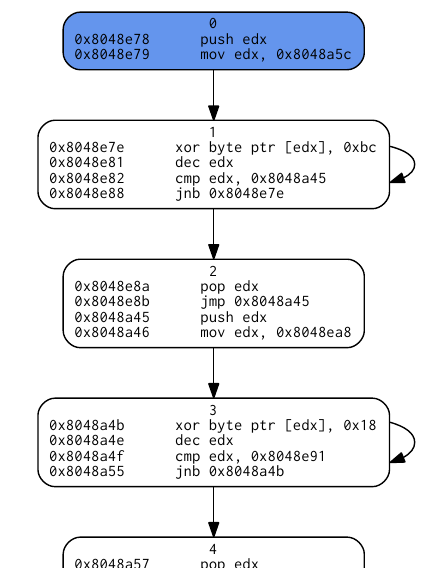
\includegraphics[width=1.0\textwidth,keepaspectratio]{first_blocks.png}
    \caption{First $2$ \texttt{xor} decryption loops}
    \label{fig:first2blocks}
  \end{subfigure}%
  \begin{subfigure}[b]{0.5\textwidth}
    \centering
    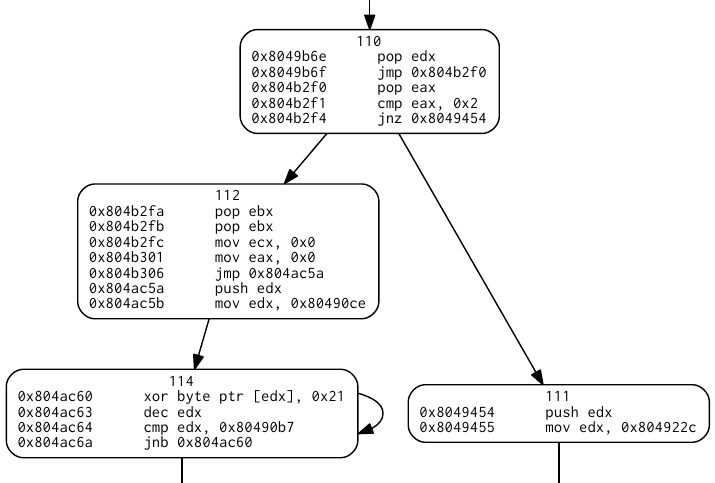
\includegraphics[width=1.0\textwidth,keepaspectratio]{check_param.png}
    \caption{Instructions check number of input arguments}
    \label{fig:checkparams}
  \end{subfigure}
  \caption{Initial analysis}
\end{figure}

A direct black-box attack (e.g. using \texttt{perf} to count the number of executed instructions when the crackme consumes an input string\footnote{See the script of \emph{jvoisin} at \url{https://dustri.org/b/defeating-the-recons-movfuscator-crackme.html}}) does not seem to be working: if input is any printable character then the number of executed instructions is always $40681$.

\section{Differential analysis}
We develop in Binsec project~\autocite{binsec} a Pin-based~\autocite{LukCMPKLWRH05} tracing tool with powerful functionalities, we use here only a simple one: tracing the list of executed instructions and some concrete information of each instruction: read/write values on registers and memory addresses.

Let's tracing the crackme with two different inputs, e.g. ``a'' and ``Ab'', observing the difference between two traces (both of them are of length $40681$),  \emph{we understand immediately the trick}. Since the instructions used in \texttt{xor} decryption loops are identical in both traces, the only difference is at the execution of instructions handling the input.~\Cref{fig:firstdiff} shows the first difference, we recognize immediately that the first byte of input string is xored with $0\mathtt{x}41$. There are $28$ such a difference, next is a comparison to check whether the $29$-th input character is $0$ or not, so we can guess that the good input should have length $28$; tracing the crackme with an input of length $28$ confirms this guess (see~\Cref{fig:checkinput}). 

\begin{figure}[ht]
  \centering
  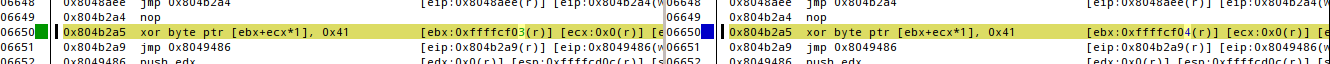
\includegraphics[width=1.0\textwidth,keepaspectratio]{compare_first.png}
  \caption{Difference reveals interesting instruction}
  \label{fig:firstdiff}
\end{figure}

\begin{figure}[ht]
  \centering
  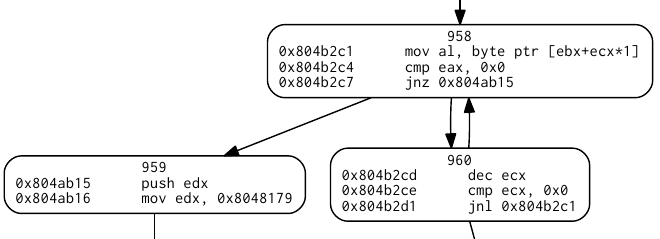
\includegraphics[width=0.5\textwidth,keepaspectratio]{check_input.png}
  \caption{Check input length and value}
  \label{fig:checkinput}
\end{figure}

We observe also in the loop in~\Cref{fig:checkinput} that, if the input length is $28$ then each byte of xored input string is compared with $0$. The \texttt{OCaml} program in~\Cref{lst:keygen} calculates an input string based on $28$ differences observed, it gives the key \texttt{Alph4t3stf0rc3mille!!!!!!!!!}, using this key as the input for crackme we get \texttt{Well done!}.

\begin{lstlisting}[frame=single, caption={Calculate good input}, captionpos=b, boxpos=b, language=Caml, label=lst:keygen]
let () =
  let () = Printf.printf "reverseMe key: " in
  let key_chars = ['\x41'; '\x6c'; '\x70'; '\x68'; '\x34'; '\x74'; '\x33';
                   '\x73'; '\x74'; '\x66'; '\x30'; '\x72'; '\x63'; '\x33';
                   '\x6d'; '\x69'; '\x6c'; '\x6c'; '\x65'; '\x21'; '\x21';
                   '\x21'; '\x21'; '\x21'; '\x21'; '\x21'; '\x21'; '\x21']
  in
  List.iter (fun ch -> Printf.printf "%c" ch) key_chars
\end{lstlisting}


% \begin{figure}[ht]
%   \centering
%   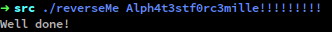
\includegraphics[width=0.5\textwidth,keepaspectratio]{reverseMe.png}
%   \caption{Good input}
%   % \label{fig:checkinput}
% \end{figure}

\section{Conclusion}
This is very nice crackme, using the same principle, we think that the author can give more difficult challenges (for this case, we get the good input in about $30-40$ minutes). It may be interesting that our \emph{concolic execution engine}~\autocite{binsec} can solve this crackme almost immediately. Our approach is similar with one of our friend Aurélien of Airbus team, he has used directly \texttt{gdb} to get the trace, so this is much more cool \smiley{}. 
 % give the detail analysis just to understand how the crackme works
% It may worth noting that the black box attack will work once we know the length of correct input message (which is $28$): 

\printbibliography

\end{document} 